% --------------------------------------------------------------
% This is all preamble stuff that you don't have to worry about.
% Head down to where it says "Start here"
% --------------------------------------------------------------
 
\documentclass[12pt]{article}
 
\usepackage[margin=1in]{geometry} 
\usepackage{amsmath,amsthm,amssymb,scrextend}
\usepackage{fancyhdr}
\usepackage{enumitem}
\usepackage{amsmath}
\usepackage{amssymb}
\usepackage{textcomp}
\usepackage{fancybox}
\usepackage{tikz}
\usepackage{tasks}
\pagestyle{fancy}
\usepackage[makeroom]{cancel}
\usepackage{graphicx}
\usepackage{caption}
\usepackage{mwe}


\usepackage{tikz}
\usetikzlibrary{positioning}

\newenvironment{rcases}
  {\left.\begin{aligned}}
{\end{aligned}\right\rbrace}

\newcommand{\N}{\mathbb{N}}
\newcommand{\Z}{\mathbb{Z}}
\newcommand{\I}{\mathbb{I}}
\newcommand{\R}{\mathbb{R}}
\newcommand{\Q}{\mathbb{Q}}
\renewcommand{\qed}{\hfill$\blacksquare$}
\let\newproof\proof
\renewenvironment{proof}{\begin{addmargin}[1em]{0em}\begin{newproof}}{\end{newproof}\end{addmargin}\qed}
% \newcommand{\expl}[1]{\text{\hfill[#1]}$}
 
\newenvironment{theorem}[2][Theorem]{\begin{trivlist}
\item[\hskip \labelsep {\bfseries #1}\hskip \labelsep {\bfseries #2.}]}{\end{trivlist}}
\newenvironment{lemma}[2][Lemma]{\begin{trivlist}
\item[\hskip \labelsep {\bfseries #1}\hskip \labelsep {\bfseries #2.}]}{\end{trivlist}}
\newenvironment{problem}[2][Problem]{\begin{trivlist}
\item[\hskip \labelsep {\bfseries #1}\hskip \labelsep {\bfseries #2.}]}{\end{trivlist}}
\newenvironment{exercise}[2][Exercise]{\begin{trivlist}
\item[\hskip \labelsep {\bfseries #1}\hskip \labelsep {\bfseries #2.}]}{\end{trivlist}}
\newenvironment{reflection}[2][Reflection]{\begin{trivlist}
\item[\hskip \labelsep {\bfseries #1}\hskip \labelsep {\bfseries #2.}]}{\end{trivlist}}
\newenvironment{proposition}[2][Proposition]{\begin{trivlist}
\item[\hskip \labelsep {\bfseries #1}\hskip \labelsep {\bfseries #2.}]}{\end{trivlist}}
\newenvironment{corollary}[2][Corollary]{\begin{trivlist}
\item[\hskip \labelsep {\bfseries #1}\hskip \labelsep {\bfseries #2.}]}{\end{trivlist}}




\setlength{\parindent}{0pt}
\begin{document}
\setcounter{section}{3}

 \settasks{
	counter-format=(tsk[r]),
	label-width=4ex
}
% --------------------------------------------------------------
%                         Start here
% --------------------------------------------------------------

\lhead{Math 475}
\chead{Chapter 4}
\rhead{Meenmo K.}

\section{Generating Permutations and Combinations}
\subsection{Generating Permutation}
{\bf Potentially useful formula} Sterling's Formula
$$n!\sim \sqrt{2\pi n}\left(\frac{n}{e}\right)^n$$

\underline{Idea} We can write down all the permutations of $n$ objects by "weaving" $n$ across the permutations of $n-1$ objects.\\

{\sl Example}(p.90)
$$\includegraphics{Lecture/chp4_image.png}$$

Algorithm for generating permutations of \{1, 2, ..., n\}
\begin{itemize}
    \item Start with $\overleftarrow{1} \overleftarrow{2} \ldots \overleftarrow{n}$\\
    (A mobile integer is one whose arrow points to an adjacent smaller integer.)
    
    \begin{enumerate}
        \item Find the largest mobile integer $m$. 
        \item Switch $m$ with the adjacent integer that its arrow points to.
        \item Switch the direction of all arrows above integers $p$ with $p>m$.
    \end{enumerate}
\end{itemize}

{\sl Example} n=4
$$\overleftarrow{1}\overleftarrow{2}\overleftarrow{3}\overleftarrow{4}$$
$$\overleftarrow{1}\overleftarrow{2}\overleftarrow{4}\overleftarrow{3}$$
$$\overleftarrow{1}\overleftarrow{4}\overleftarrow{2}\overleftarrow{3}$$
$$\overleftarrow{4}\overleftarrow{1}\overleftarrow{2}\overleftarrow{3}$$
$$\overrightarrow{4}\overleftarrow{1}\overleftarrow{3}\overleftarrow{2}$$
$$\overleftarrow{1}\overrighttarrow{4}\overleftarrow{3}\overleftarrow{2}$$
$$\overleftarrow{1}\overleftarrow{3}\overrightarrow{4}\overleftarrow{2}$$
$$\overleftarrow{1}\overleftarrow{3}\overleftarrow{2}\overrightarrow{4}$$
$$\overleftarrow{3}\overleftarrow{1}\overleftarrow{2}\overleftarrow{4}$$
$$\vdots$$
$$\text{until}$$
$$\overleftarrow{2}\overleftarrow{1}\overrightarrow{3}\overrightarrow{4}$$
$$\text{Nothing mobile, so we stop!}$$

\vspace{2\baselineskip}
\subsection{Inversions in Permutations}
Let $i_1i_2i_3\ldots i_n$ be a permutation of \{1,2,\ldots,n\}. An \underline{inversion} is a pair $(i_k,\;i_l)$ such that $k<l$ but $i_k>i_l$.\\

{\sl Example } 6 3 5 1 2 4 has inversions
\begin{align*}
    &(6,3) & (3,1) & (5,1)\\
    &(6,5) & (3,2) & (5,2)\\
    &(6,1) &     & (5,4)\\
    &(6,1) &     &\\
    &(6,2) &     &\\
    &(6,4) &     &
\end{align*}
There are 10 total inversions. \\

For the permutation $i_1i_2i_3\ldots i_n$, let $a_j$ be the number of inversions whose second component is $j$. The sequence $a_1a_2a_3\ldots a_n$ is called the \underline{inversion sequence}. ($a_j$ equals the number of integers that precede $j$ in the permutation that are greater than $j$).\\

{\sl Example} $a_1=3\quad a_2=3\quad a_3=1\quad a_4=2\quad a_5=1\quad a_6=0$
So, the permutation 6 3 5 1 2 4 has inversion sequence 3 3 1 2 1 0.\\

{\bf Theorem 4.2.1} Let $b_1,\;b_2,\;...,b_n$ be integers satisfying $$0\le b_1\le n-1,\;0\le b_2\le n-2,\;0\le b_{n-1}\le 1,\; b_n=0$$. Then there is a unique permutation whose inversion sequence is $b_1b_2\ldots b_n$.\\

{\sl Proof} Use an algorithm (see pp.94-96 of Brualdi for details)\\
Let 5 1 4 3 0 1 1 0 be an inversion sequence.\\

\underline{Algorithm I} (right to left):\\ 
Each $b_k$ tells us how many entries in permutation bigger than $k$ precede $k$.
$$8$$
$$87$$
$$867$$
$$5867$$
$$58647$$
$$586437$$
$$5286437$$
$$52864137$$\\

\underline{Algorithm II} (left to right):\\
Place each $k$ in open spot $b_k+1$
\begin{center}
    


\tikzset{every picture/.style={line width=0.75pt}} %set default line width to 0.75pt        

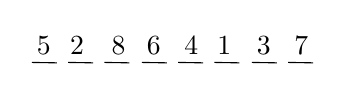
\begin{tikzpicture}[x=0.75pt,y=0.75pt,yscale=-1,xscale=1]
%uncomment if require: \path (0,423.0242919921875); %set diagram left start at 0, and has height of 423.0242919921875

%Straight Lines [id:da0016498639377078295] 
\draw    (247.25,119) -- (259.3,119.2) ;


%Straight Lines [id:da9355290820987332] 
\draw    (300.22,119) -- (312.27,119.2) ;


%Straight Lines [id:da9046454469286882] 
\draw    (317.68,119) -- (329.73,119.2) ;


%Straight Lines [id:da9461721157719922] 
\draw    (264.71,119) -- (276.76,119.2) ;


%Straight Lines [id:da16909459182226838] 
\draw    (282.17,119) -- (294.22,119.2) ;


%Straight Lines [id:da34738665894772836] 
\draw    (353.19,119) -- (365.24,119.2) ;


%Straight Lines [id:da7224719279116638] 
\draw    (370.65,119) -- (382.7,119.2) ;


%Straight Lines [id:da12588819868684586] 
\draw    (335.14,119) -- (347.19,119.2) ;



% Text Node
\draw (253,111) node  [align=left] {5};
% Text Node
\draw (306,111) node  [align=left] {6};
% Text Node
\draw (269,111) node  [align=left] { 2};
% Text Node
\draw (340,111) node  [align=left] {1};
% Text Node
\draw (359,111) node  [align=left] {3};
% Text Node
\draw (377,111) node  [align=left] {7};
% Text Node
\draw (324,111) node  [align=left] {4};
% Text Node
\draw (289,111) node  [align=left] {8};
\end{tikzpicture}
\end{center}

\subsection{Generating Combinations}
{\sl Goal} Given a set of $n$ distinct elements, write down all $2^n$ subsets of our set.\\

{\sl Approach} count n-digit binary integers.\\
\underline{Ex} n=4\quad S=\{A, B, C, D\}\quad $0\le k\le 2^n-1$
\begin{center}
\begin{tabular}{ccc}
\textbf{k} & \textbf{\begin{tabular}[c]{@{}c@{}}n-bit\\ binary representation of k\end{tabular}} & \textbf{subset of S} \\
0          & 0000                                                                                & $\phi$               \\
1          & 0001                                                                                & \{A\}                \\
2          & 0010                                                                                & \{B\}                \\
3          & 0011                                                                                & \{A,B\}              \\
4          & 0100                                                                                & \{C\}                \\
5          & 0101                                                                                & \{A,C\}              \\
6          & 0110                                                                                & \{B,C\}              \\
7          & 0111                                                                                & \{A,B,C\}            \\
8          & 1000                                                                                & \{D\}                \\
9          & 1001                                                                                & \{A,D\}              \\
10         & 1010                                                                                & \{B,D\}              \\
11         & 1011                                                                                & \{A,B,D\}            \\
12         & 1100                                                                                & \{C,D\}              \\
13         & 1101                                                                                & \{A,C,D\}\\    
14         & 1110                                                                                & \{B,C,D\}              \\
15         & 1111                                                                                & \{A,B,C,D\}           
\end{tabular}
\end{center}
This ordering is called \underline{lexicographic} ordering of the sequence of 0s and 1s.\\

The order of the third column 'subset of S' is called the \underline{squashed order}.

\subsection{Generating r-subsets}
Recall the squashed order of the subsets of \{A,B,C,D\}. 
\begin{center}
    \begin{tabular}{cccll}
    {0}            & {0}            & {0}            &  & $\phi$    \\
    {0}            & 0                     & 1                     &  & \{A\}     \\
    {0}            & 1                     & 0                     &  & \{B\}     \\
    {0}            & 1                     & 1                     &  & \{A,B\}   \\
    {1}            & 0                     & 0                     &  & \{C\}     \\
    1                     & 0                     & 1                     &  & \{A,C\}   \\
    \multicolumn{1}{l}{1} & \multicolumn{1}{l}{1} & \multicolumn{1}{l}{0} &  & \{B,C\}   \\
    \multicolumn{1}{l}{1} & \multicolumn{1}{l}{1} & \multicolumn{1}{l}{1} &  & \{A,B,C\}
    \end{tabular}
\end{center}
2-subsets: \{A,B\}, \{A,C\}, \{B,C\} $\Rightarrow$ squashed ordering of 2-subsets inherited from the squashed ordering of all subsets.\\

{\sl Example} Squashed order of 2-subsets of \{A,B,C,D\} is 
$$\{A,B\}\quad\{A,C\}\quad\{A,D\}$$
$$\{B,C\}\quad\{B,D\}\quad\{C,D\}$$\\

{\sl Big Idea} Lexicographic order is essentially alphabetic order.\\

{\sl Example} Lexicographic order of 3-subsets of \{1,2,3,4,5\} (should be $\binom{5}{3}=10$ of these)
\begin{center}
    \begin{tabular}{cccllll}
        1 & 2 & 2 &  & 1 & 4 & 5 \\
        1 & 2 & 4 &  & 2 & 3 & 4 \\
        1 & 2 & 5 &  & 2 & 3 & 5 \\
        1 & 3 & 4 &  & 2 & 4 & 5 \\
        1 & 3 & 5 &  & 3 & 4 & 5
        \end{tabular}
\end{center}
\end{document}